\section{Project Structure}

We use, as already mentioned, two GIT repositories, LpzRobots and GoRobots. A rough overview of the structure is given below in Figure \ref{struc}:


Later, the controllers for each robot will be implemented within \emph{GoRobots}, accessing the robots, which are located in \emph{LpzRobots}. The folder \emph{DEMO} will later contain demos of the different robots.
Another visualisation of the two repositories and where which file belongs is given in Figure \ref{struc2}. 
\begin{figure}[h!]
 \begin{center}
  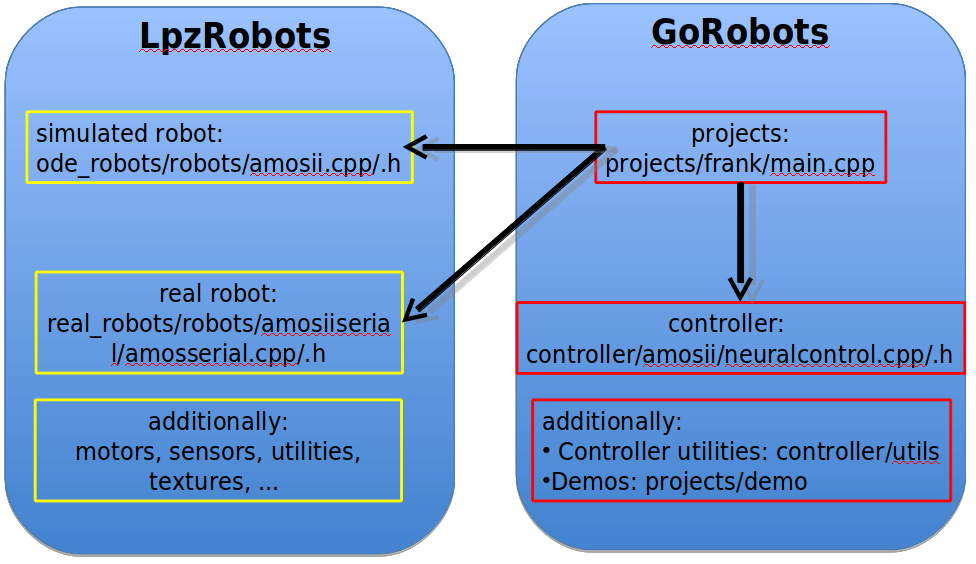
\includegraphics[width=10cm]{./Pics/struct.png}
 \end{center}
\caption{Structure of the two repositories, LpzRobots and GoRobots}
\label{struc2}
\end{figure}

You will later work with your own copy of the two repositories.

\newpage

\begin{figure}[h!]
 \begin{center}
  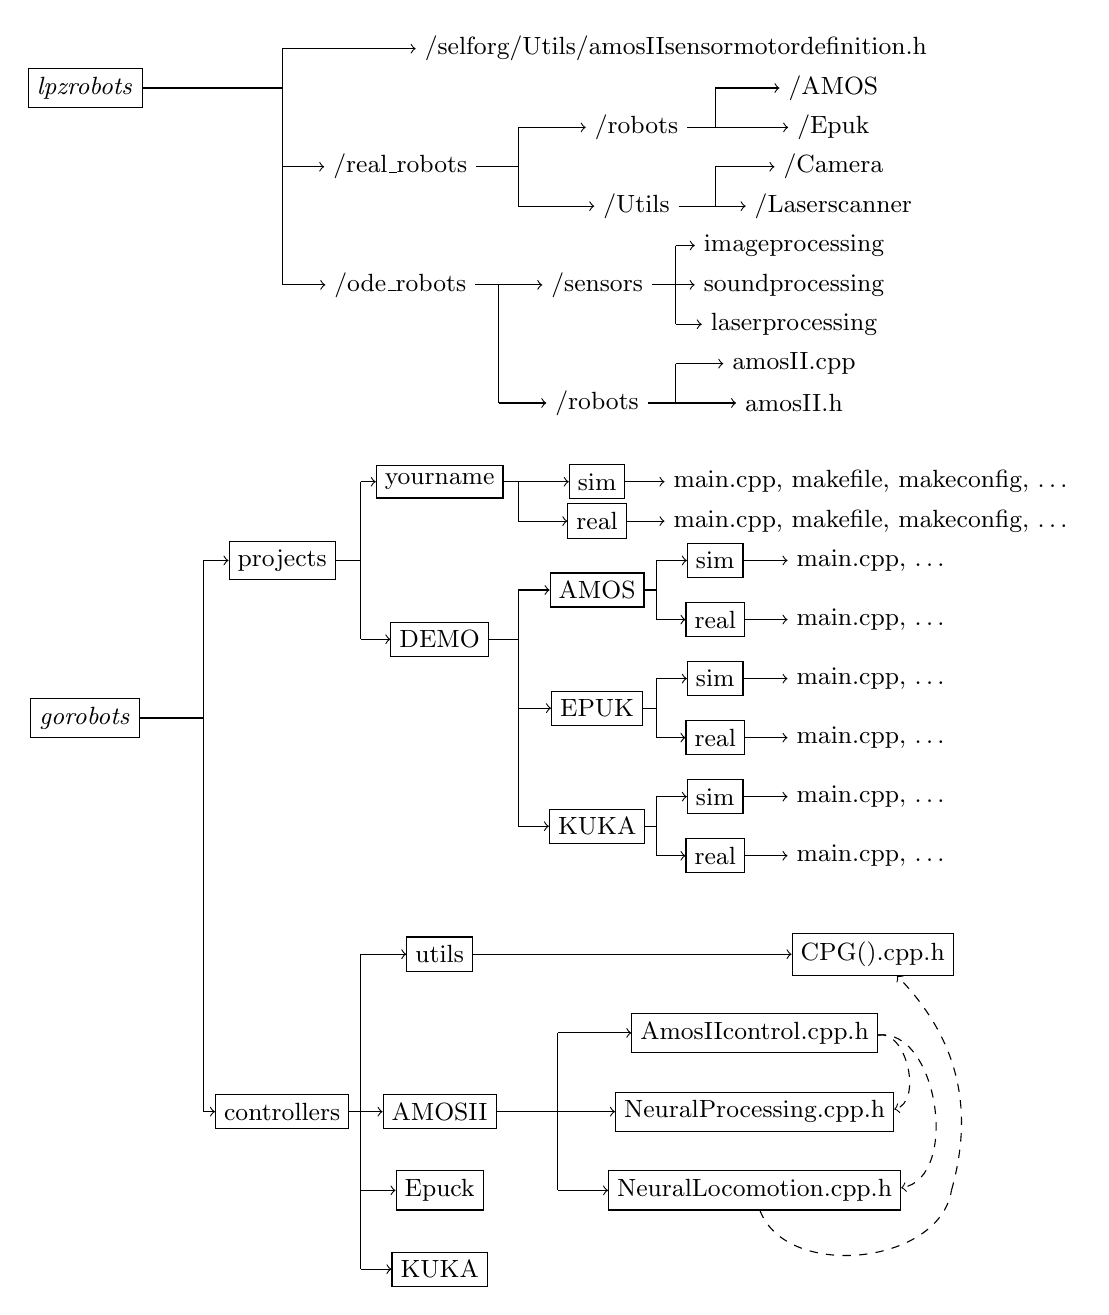
\begin{tikzpicture}{gitbranches}
   \small
  \node at (-1,-2) (lpz) [rectangle,draw] {\emph{lpzrobots}};
  \node at (3,-3) (realR) [] {/real\_robots};
  \node at (6.5,-1.5) (selforg) [] {/selforg/Utils/amosIIsensormotordefinition.h};
  \node at (3,-4.5) (odeR) [] {/ode\_robots};
  \node at (5.5,-4.5) (sensors) [] {/sensors};
  \node at (5.5,-6) (robots) [] {/robots};
  \node at (8,-4) (IP) [] {imageprocessing};
  \node at (8,-4.5) (SP) [] {soundprocessing};
  \node at (8,-5) (P) [] {laserprocessing};
  \node at (8,-5.5) (ACPP) [] {amosII.cpp};
  \node at (8,-6) (AH) [] {amosII.h};

\node at (6, -2.5) (RRrobots) [] {/robots};
\node at (6, -3.5) (RRutils) [] {/Utils};

\node at (8.5, -2) (RRamos) [] {/AMOS};
\node at (8.5, -2.5) (RRepuk) [] {/Epuk};

\node at (8.5, -3) (RRcamera) [] {/Camera};
\node at (8.5, -3.5) (RRlsc) [] {/Laserscanner};


   \path[->]
	      ( 1.5,-3) edge (realR)
	      ( 1.5,-1.5) edge (selforg)
	      ( 1.5,-4.5) edge (odeR)
	      (4.25,-4.5) edge (sensors)
	      (4.25,-6) edge (robots)
	      (6.5,-4) edge (IP)
	      (6.5,-4.5) edge (SP)
	      (6.5,-5) edge (P)
	      (6.5,-5.5) edge (ACPP)
	      (6.5,-6) edge (AH)
	      (4.5, -2.5) edge (RRrobots)
	      (4.5, -3.5) edge (RRutils)
	      (7, -2) edge (RRamos)
	      (7, -2.5) edge (RRepuk)
	      (7, -3) edge (RRcamera)
	      (7, -3.5) edge (RRlsc)
	      ;
  \path[-]
	      (lpz) edge ( 1.5,-2)
	      (1.5,-1.5) edge (1.5,-4.5)
	      (odeR) edge (4.25,-4.5)
	      (4.25,-4.5) edge (4.25, -6)
	      (sensors) edge (6.5,-4.5)
	      (robots) edge (6.5,-6)
	      (6.5,-4) edge (6.5,-5)
	      (6.5, -5.5) edge (6.5,-6)
	      (realR) edge (4.5,-3)
	      (4.5, -2.5) edge ( 4.5, -3.5)
	      (RRrobots) edge (7, -2.5)
	      (7, -2) edge (7, -2.5)
	      (RRutils) edge (7, -3.5)
	      (7, -3) edge (7, -3.5)
	      ;


   \node at (-1,-10) (gorobots) [rectangle,draw] {\emph{gorobots}};
   \node at (1.5,-8) (projects) [rectangle,draw] {projects};
   \node at (1.5,-15) (controllers) [rectangle,draw] {controllers};
   \node at (3.5,-7) (yn) [rectangle,draw] {yourname};
   \node at (3.5,-9) (demo) [rectangle,draw] {DEMO};
   \node at (5.5,-7) (sim) [rectangle,draw] {sim};
   \node at (5.5,-7.5) (real) [rectangle,draw] {real};

   \node at (9,-7) (simS) [] {main.cpp, makefile, makeconfig, \ldots};
   \node at (9,-7.5) (realS) [] {main.cpp, makefile, makeconfig, \ldots};
   
    \node at (5.5, -8.375) (AMOS) [draw] {AMOS};
    \node at (5.5, -9.875) (EPUK) [draw] {EPUK};    
    \node at (5.5, -11.375) (KUKA) [draw] {KUKA};

    \node at (7,-8) (AMOSsim) [draw] {sim};
    \node at (9,-8) (AMOSsimS) [] {main.cpp, \ldots};
    \node at (7,-8.75) (AMOSreal) [draw] {real};
    \node at (9,-8.75) (AMOSrealS) [] {main.cpp, \ldots};
    \node at (7,-9.5) (EPUKsim) [draw] {sim};
    \node at (9,-9.5) (EPUKsimS) [] {main.cpp, \ldots};
    \node at (7,-10.25) (EPUKreal) [draw] {real};
    \node at (9,-10.25) (EPUKrealS) [] {main.cpp, \ldots};
    \node at (7,-11) (KUKAsim) [draw] {sim};
    \node at (9,-11) (KUKAsimS) [] {main.cpp, \ldots};
    \node at (7,-11.75) (KUKAreal) [draw] {real};
    \node at (9,-11.75) (KUKArealS) [] {main.cpp, \ldots};

    \node at (3.5,-13) (utils) [draw] {utils};
    \node at (3.5,-15) (AMOSII) [draw] {AMOSII};
    \node at (9,-13) (AMOSCPG) [draw] {CPG().cpp.h};
    \node at (3.5,-16) (EPUKCon) [draw] {Epuck};
    \node at (3.5,-17) (KUKACon) [draw] {KUKA};


    \node at (7.5,-14) (AMOSIICon) [draw] {AmosIIcontrol.cpp.h};
    \node at (7.5,-15) (AMOSIINP) [draw] {NeuralProcessing.cpp.h};
    \node at (7.5,-16) (AMOSIINL) [draw] {NeuralLocomotion.cpp.h};

\draw[dashed,bend left=89, ->] (AMOSIICon) to (AMOSIINP);
\draw[dashed,bend left=89, ->] (AMOSIICon) to (AMOSIINL);


   \path[->]
    (0.5,-8) edge (projects)
    (0.5,-15) edge (controllers)
    (2.5,-7) edge (yn)
    (2.5, -9) edge (demo)
    (4.5,-7) edge (sim)
    (4.5,-7.5) edge (real)
    (sim) edge (simS)
    (real) edge (realS)
    (4.5, -8.375) edge (AMOS)
    (4.5, -9.875) edge (EPUK)
    (4.5, -11.375) edge (KUKA)
    (6.25, -8) edge (AMOSsim)
    (6.25, -8.75) edge (AMOSreal)
    (6.25, -9.5) edge (EPUKsim)
    (6.25, -10.25) edge (EPUKreal)
    (6.25, -11) edge (KUKAsim)
    (6.25, -11.75) edge (KUKAreal)
    (AMOSsim) edge (AMOSsimS)
    (AMOSreal) edge (AMOSrealS)
    (EPUKsim) edge (EPUKsimS)
    (EPUKreal) edge (EPUKrealS)
    (KUKAsim) edge (KUKAsimS)
    (KUKAreal) edge (KUKArealS)
    (utils) edge (AMOSCPG)
    (2.5,-13) edge (utils)
    (2.5,-15) edge (AMOSII)
    (2.5, -16) edge (EPUKCon)
    (2.5,-17) edge (KUKACon)
    (5,-14) edge (AMOSIICon)
    (5,-15) edge (AMOSIINP)
    (5,-16) edge (AMOSIINL)
    ;

   \path[-]
    (gorobots) edge (0.5,-10)
    (0.5,-8) edge (0.5,-15)
    (projects) edge ( 2.5,-8)
    (2.5, -7) edge (2.5, -9)
    (yn) edge (4.5, -7)
    (4.5,-7) edge (4.5,-7.5)
    (demo) edge (4.5,-9)
    (4.5, -8.375) edge (4.5,-11.375)
    (AMOS) edge (6.25,-8.375)
    (EPUK) edge (6.25,-9.875)
    (KUKA) edge (6.25,-11.375)
    (6.25,-8) edge (6.25,-8.75)
    (6.25,-9.5) edge (6.25,-10.25)
    (6.25,-11) edge (6.25,-11.75)
    (controllers) edge (2.5,-15)
    (2.5,-13) edge (2.5,-17)
    (AMOSII) edge (5,-15)
    (5,-14) edge (5,-16)
    
    ;
\draw[dashed,bend right=75] (AMOSIINL) to (10,-16);
\draw[dashed, ->, bend right] (10,-16) to (AMOSCPG);

% \draw (AMOSIINL) to [bend right] (AMOSCPG) node {};


\end{tikzpicture}
 \end{center}
\caption{Structure of the two repositories, LpzRobots and GoRobots}
\label{struc}
\end{figure}